%%%%%%%%%%%%%%%%%%%%%%%%%%%%%%%%%%%%%%%%
% basic elements

\documentclass[12pt]{article}
\usepackage[english]{babel}
\usepackage{amsmath,amsthm}
\usepackage{amsfonts}
\usepackage{makecell}
\usepackage{graphics}
\usepackage{graphicx}
\usepackage{fancyhdr}
\usepackage{ifthen}
\usepackage{wrapfig}
\usepackage{array}
\usepackage{colortbl}
\usepackage{fullpage}
\usepackage[table]{xcolor}
\usepackage{subfigure}
\usepackage{caption}
\usepackage{float}
\usepackage{ctex}
\usepackage{appendix}
\usepackage{shorttoc}
\usepackage{pagenote}
\usepackage{setspace}
\usepackage{geometry}
\usepackage{indentfirst}
\usepackage{fullpage}
\usepackage{booktabs}
\usepackage{multirow}
\usepackage{longtable}
\usepackage{minipage-marginpar}
\usepackage{hyperref}
\usepackage{palatino}
\usepackage{setspace}
\usepackage{subfigure}
\usepackage{picinpar}
\usepackage{newtxtext}
\usepackage{amsmath,amssymb,amsthm}
\usepackage{extarrows}
\usepackage{algorithm}
\usepackage{algorithmic}
\usepackage{newtxmath} % must come after amsXXX

% Replace ABCDEF in the next line with your chosen problem
% and replace 111111 with your Team Control Number
% and replace abcdef with your Title
% and replace 123456 with the number of pages of your essay
\newcommand{\Problem}{A}
\newcommand{\Team}{{22091106}}
\newcommand{\Title}{{Smart Lamppost Deployment}}
\newcommand{\wholepages}{20}
\title{\huge\textbf{\Title}}
\author{Team\#\Team}
\date{\today}

%%%%%%%%%%%%%%%%%%%%%%%%%%%%%%%%%%%%%%%%
% set up of theorems

\newtheorem{thm}{Theorem}[section]
\newtheorem{cor}[thm]{Corollary}
\newtheorem{lem}[thm]{Lemma}
\newtheorem{prop}[thm]{Proposition}
\theoremstyle{definition}
\newtheorem{defn}[thm]{Definition}
\theoremstyle{remark}
\newtheorem{rem}[thm]{Remark}
\numberwithin{equation}{section}
\newtheorem{theorem}{Theorem}
\newtheorem{corollary}[theorem]{Corollary}
\newtheorem{lemma}[theorem]{Lemma}
\newtheorem{definition}{Definition}

%%%%%%%%%%%%%%%%%%%%%%%%%%%%%%%%%%%%%%%%
% setup of page length and script size

\setlength{\belowcaptionskip}{9pt}
\setlength{\abovecaptionskip}{9pt}
\setlength{\headsep}{0.4in}
\setlength{\headheight}{14.5pt}
\captionsetup{font={footnotesize}}
\renewcommand{\baselinestretch}{1.05}
\geometry{bottom=1in}

%%%%%%%%%%%%%%%%%%%%%%%%%%%%%%%%%%%%%%%%
% set up of page style

\pagestyle{fancy}
\fancyhead[L]{Team\ \#\Team}
\fancyhead[C]{\Title}
\fancyhead[R]{Page \thepage \ of \wholepages}
\fancyfoot{}

%%%%%%%%%%%%%%%%%%%%%%%%%%%%%%%%%%%%%%%%
% hyphenation

\tolerance=1
\emergencystretch=\maxdimen
\hyphenpenalty=10000
\hbadness=10000

\hypersetup{hidelinks} 
\hypersetup{
	colorlinks=false,
	linkcolor=black,
	citecolor=black,
	anchorcolor=black
}
%%%%%%%%%%%%%%%%%%%%%%%%%%%%%%%%%%%%%%%%
% biblography
\bibliographystyle{plain}
% \usepackage{url}
% \def\UrlBreaks{[\do\A\do\B\do\C\do\D\do\E\do\F\do\G\do\H\do\I\do\J\do\K\do\L\do\M\do\N\do\O\do\P\do\Q\do\R\do\S\do\T\do\U\do\V\do\W\do\X\do\Y\do\Z\do\[\do\\\do\]\do\^\do\_\do\`\do\a\do\b\do\c\do\d\do\e\do\f\do\g\do\h\do\i\do\j\do\k\do\l\do\m\do\n\do\o\do\p\do\q\do\r\do\s\do\t\do\u\do\v\do\w\do\x\do\y\do\z\do\.\do\@\do\\\do\/\do\!\do\_\do\|\do\;\do\>\do\]\do\)\do\,\do\?\do\'\do+\do\=\do\#}

%%%%%%%%%%%%%%%%%%%%%%%%%%%%%%%%%%%%%%%%
% end of the beginning part
\begin{document}
	\DeclareGraphicsExtensions{.pdf, .jpg, .tif, .png}
	\thispagestyle{empty}
	\vspace*{-16ex}
	% MCM/ICM Template
	% \centerline{\begin{tabular}{*3{c}}
			%	\parbox[t]{0.3\linewidth}{\begin{center}\textbf{Problem Chosen}\\ \Large \Problem\end{center}}
			%	& \parbox[t]{0.3\linewidth}{\begin{center}\textbf{2020\\ MCM \\ Summary Sheet}\end{center}}
			%	& \parbox[t]{0.3\linewidth}{\begin{center}\textbf{Team Control Number}\\ \Large Team \# \Team\end{center}}	\\
			%	\hline
			%\end{tabular}}
	
	% HiMCM/IMMC Template
	\begin{center}
		\centerline{\begin{tabular}{p{\linewidth}<{\centering}}
				\small Team Control Number \\
				\huge \textbf{\Team} \\
				\small Problem Chosen \\
				\huge \textbf{\Problem} \\
				\textbf{2022} \\
				\small \textbf{IMMC} \\
				\small \textbf{Summary Sheet} \\
				\hline
		\end{tabular}}
	\end{center}
	%%%%%%%%%%% Begin Summary %%%%%%%%%%%%%%%%%%
	% Enter your summary here replacing the (red) text
	% Replace the text from here ...
	\qquad
	\par
	Nowadays, with the rapid development of autonomous driving technology, building a automatic driving system will no longer be a rediculous thought. In this system, connections can be built between the autonomous driving cars, the smart lampposts installed with sensors and communication units and the cloud server. So we need to carry out a plan which will make the transportation system easier and create an indicator system to evaluate the smart lamppost modification plans.
	
	In the first model, we find out the factors that is related to evaluating a lamppost modification plan. We mainly discuss how to calculate the index which is affected by cost, coverage rate of LiDar and the importance of each road. Afterwards, we make some plans about the measure of coverage rate in different situations.

	
	% to here
	%%%%%%%%%%% End Summary %%%%%%%%%%%%%%%%%%%
	\thispagestyle{empty}
	\maketitle
	\thispagestyle{empty}
	\newpage
	%%%%%%%%%%%%%%%%%%%%%%%%%%%%%%%%%%%%%%%%
	\clearpage
	\thispagestyle{empty}
	% Uncomment the next line to generate a Table of Contentsr%r%\shortableofcontents{Contents}{2}
	\tableofcontents % Uncomment this line to update the Contents
	\newpage
	\pagestyle{fancy}
	\setcounter{page}{1}
	% Begin your paper here
	%%%%%%%%%%%%%%%%%%%%%%%%%%%%%%%%%%%%%%%%
	
	\newpage
	\section{Introduction}
		\subsection{Background}
		Nowadays, with the rapid development of autonomous driving technology, building a automatic driving system will no longer be a rediculous thought. Based on recent technology, autonomous driving technology has begun to move from partial drving at the L2 level to conditional driving automation at the L3 level.
		
		According to the degree of automation of the vehicle\cite{Autonomous Driving Levels}, when the system cannot withstand the working conditions, the driver needs to take over the malfunctioning vehicle. After activating the automatic driving system, the vehicle itself can complete tasks such as steering, acceleration, deceleration, and reaction. The status detection and reaction are carried out under the operating conditions specified by the automatic driving system.
		
		In order to facilitate vehicles which will better implement the L3 level autonomous driving tasks, using smart lampposts as the main representative of the smart roadside infrastructure. By refitting existing ordinary lampposts into smart lammposts equipped with sensors and communication units. They can collect road data through sensors and upload them onto the cloud server, and then download to the original lamppost or share it with other ones after the server completes the calculations. The autonomous driving cars can obtain the road data by communicating with neighboring smart lampposts.
		\subsection{Problem Restatement}
		\begin{center}
			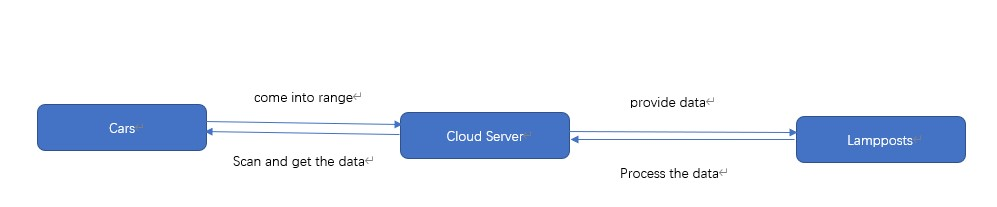
\includegraphics[width=14cm]{diagram.jpg}
			
			\small \textit{Fig. 1}
			
		\end{center}
		In this model, we actually need to have some detailed information about the whole transportation system in the area. In addition, we need to know about the driving pattern of the cars to make further dicoveries about the autonomous driving system. In Fig. 1, we can clearly discover the relationship between the car, the lamppost and the cloud server.
		
		So the problem is divided into 3 main parts:
		\begin{itemize}
			\item Build a framework for evaluating the smart lamppost modification plans based on cost and coverage of the road by the sensor and the WiFi communication.
			\item Give a plan for smart lamppost modification in an area of any city.
			\item Evaluate the lamppost modification plan based on our model and find the strengths and weaknesses of our model.
		\end{itemize}
		\subsection{General Assumptions}
		\begin{itemize}
			\item \textbf{All the cars have the same scale.}
			
			We assume that all the cars can be seen as a car which is 4.8m in length and 1.6m in width. This can flatten the neighborhood which we take into consideration.
			\item \textbf{The impact of buildings is not taken into consideration.}
			
			Since the distance between two roads is far from the detection zone, the buildings will not affect the detection of the road.
			\item \textbf{Vehicles drive on the left side according to the standard of HongKong.}
			\item \textbf{Neighborhood intersection is not taken into consideration.}
			\item \textbf{Most of the calculation is completed on the client side.}
			
			There are different types of car on the road. Since the cloud side can't afford such large amount of calculation, we assume that the most of it is completed on the client side.
			\item \textbf{The weather factors can be ignored.}
			\end{itemize}
	
	\newpage
	\section{Evaluation Model}	
		\subsection{Problem Overview}
		In this model, we will establish an indicator framwork for the purpose of evaluating smart lamppost modification plans. We will mainly discuss the effectiveness of the plan when it comes to normal roads and crossroads. In this model, crossroads is defined as a circle with a radius of 50m, centering at the middle of the crossing.
		\subsection{Assumption}
		\begin{itemize}
			\item \textbf{All the destinations can be detected and can be abstracted as a dot.}
		\end{itemize}
		\subsection{Notation}
		\begin{tabular}{ll}
		\hline
		Symbol&Stands For\\
		\hline
		$S$&Evaluating Index\\
		$P$&Overall Cost\\
		$a_1$&The Coverage Rate of Sensors on Crossroads\\
		$a_2$&The Coverage Rate of Sensors on Normal Roads\\
		$b_1$&The Coverage Rate of WiFi Communication on Crossroads\\
		$b_2$&The Coverage Rate of WiFi Communication on Normal Roads\\
		$k_1$&Weight of Crossroads\\
		$k_2$&Weight of Normal Roads\\
		\hline
		\end{tabular}	
		\subsection{Determining the Factors}
		For we need to think more about the crosswords, we consider the crossroads more important than normal roads. So we can infer that:
		$k_1>k_2$
		
		So we find out a simple formula describing the effectiveness of the system:
		$$S=\dfrac{k_1(a_1+b_1)+k_2(a_2+b_2)}{P}$$
		$$\left(k_1>>k_2\right)$$
		
		In this formula, $a_1$is identified as $\dfrac{S_{coverage}}{S_{all}}$, so we can easily get the formula describing $a_2$,$b_1$,$b_2$.
		
	\newpage
	\section{Model}
		\subsection{Problem Overview}
		In this model, we will focus on the smart lamppost modification plan based on the transportation system in HongKong.(The map is attached at the end of this essay.) We can abstract this map into a rectangular coordinate system.
		\begin{center}
			%\includegraphics[width=9cm]{.jpg}
			\small \textit{Fig. 2}
		\end{center}
	
		In this area, Gaoshida Evenue has a spped limit of 70km/h(19.5m/s) and other roads have a speed limit of 50km/h(14.0m/s). So speed needs to be taken into consideration.
		\subsection{Definition}
		We assume that an autonomous driving need no time to turn left and 5 second to turn right. The number comes from the calculation according to the average width of roads and the highest speed to steer safely in normal conditions. This means that when a car turn right, it will disappear immediately and appear at the end of the line in this road after 5 second. In this process, the car will exert no impact on other cars.
		So now let we assume that we are in an autonomous driving car. If the car is running normally
		\subsection{Assumptions}
		\begin{itemize}
			\item \textbf{Pedestrians are ignored in this model.}
		\end{itemize}
	\subsection{Model Simulation}
	To get further understanding of the transportation system in this area.
	
	\begin{algorithm}
		\caption{Get the State of Distribution}
		\label{Type}
		\begin{algorithmic}
		% Get\_State(Distribution):
		\STATE Cost = $5000\cdot (\text{Lampposts with only LiDAR})$\\ $+3000\cdot  (\text{Lampposts with only WiFi})$\\\par\par$+10000\cdot (\text{Lampposts with both})$
		\STATE \# Formula of calculating coverage: $\dfrac{S_{\mathrm{road\_}} \mathrm{covered}}{S_{\mathrm{roads}}}$​​
		\STATE State = $\sum_{\begin{array}{c}
				\mathrm{road} \mathrm{type}\xlongequal{\mathrm{def}}\mathrm{r}\in \left\{ \mathrm{Inter}\sec\mathrm{tion}, \mathrm{Normal} \right\}\\
				\mathrm{device}\xlongequal{\mathrm{def}}\mathrm{d}\in \left\{ \mathrm{LiDAR}, \mathrm{WiFi} \right\}\\
		\end{array}}$
		\STATE ${\frac{\mathrm{r}\cdot \mathrm{d}}{\mathrm{Cost}}}=\frac{k_1\left( a_1+b_1 \right) +k_2\left( a_2+b_2 \right)}{P}$
		\STATE return State
		\STATE L = Set of all SmartLamps
		\STATE done = False
		\STATE initialize q\_table, LEARNING\_RATE and DISCOUN
		\WHILE{not done:}
		\STATE update q\_table
		\ENDWHILE
		\FOR{lamp in L:}
		\WHILE{in attempt to change the configuration of lamp:}
		\IF{Get\_State(new\_distribution) > Get\_State(current\_distribution):}
		\STATE change distribution
		\ELSE
		\STATE remain
		\ENDIF
		\ENDWHILE
		\ENDFOR
		\STATE previous loop $\rightarrow$ find q\_table[max\_distribution] and corresponding action
		\STATE current\_distribution = q\_table[current\_state + action]
		\STATE new\_distribution = (1 - LEARNING\_RATE) * current\_distribution +\\ LEARNING\_RATE$\times$ ($\delta Get_State$ + DISCOUNT * max\_distribution)
		\STATE q\_table[current\_state + action] = new\_distribution
		\STATE conduct the loop continuously until the previous loop doesn't alter anything:
		\STATE done = True
		\end{algorithmic}
	\end{algorithm}
	
		
		
	
	
	\newpage
	\section{Evaluation of Our Own Plan}
	\subsection{Problem Overview}
	In this part, we will use our index to evaluate our plan. By getting the number and comparing it with other parts, we will find the strengths and weaknesses of our plan. Later we will show what improvements we decide to make to our model and what we can do with the development of the automatic driving system.
	\subsection{Result Analysis}
	\subsubsection*{Strength}
	\begin{itemize}
		\item \textbf{}
	\end{itemize}
	
	\subsubsection*{Weaknesses and Expectation}
	\begin{itemize}
		\item \textbf{The evaluation model is static.}
		
		In the first part, we ignore the movement of cars, this will reduce the accuracy of this model.
		\item \textbf{There is difference between our model and reality.}
		
		Nowadays, the WiFi technology is not so effecient and the calculation on the client side doesn't have such a speed as assumed in our model. Our model should make improvements. In addition, we should always pay attention to new technology while the technology is developing.
	\end{itemize}
	
	\newpage
	\thispagestyle{empty}
	\renewcommand\refname{Appendix}
	\clearpage
	\addcontentsline{toc}{section}{Appendices}
	\tolerance=500
	\begin{center}
		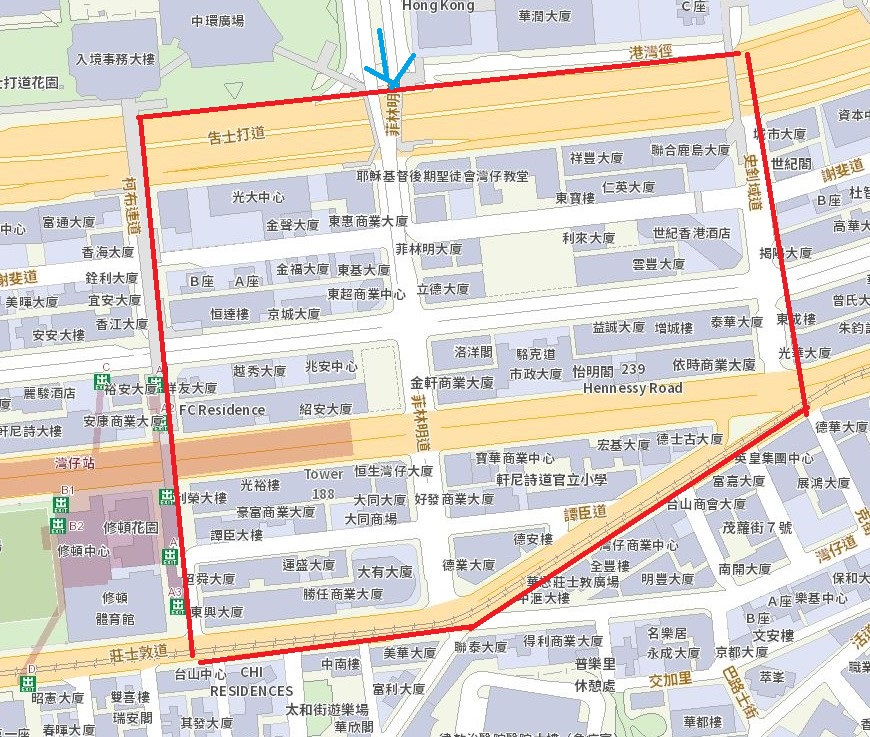
\includegraphics[width=16cm]{map.jpg}
		\small \textit{Fig. The Map of Selected City Areas }
	\end{center}
	
	
	
	
	\newpage
	\thispagestyle{empty}
	% \setcounter{page}{\wholepages}
	\renewcommand\refname{References}
	\clearpage
	\addcontentsline{toc}{section}{References}
	\tolerance=500
	\begin{thebibliography}{100}
		\bibitem {Autonomous Driving Levels}https://www.sae.org/standards/content/j3016\_201806/
		\bibitem {Map}https://www.map.gov.hk/gm/map/
		
	\end{thebibliography} 
	
\end{document}